\chapter{移动平台设计和制造}
\label{cha:Platform}

\section{平台设计}
形式:

每个小车为一个数据点,在1-3维坐标系内动态运动(如果和ShapeBots\cite{suzuki2019shapebots}一样具备升降平台或者和SwarmOS一样具备可变色LED点阵则可以进行三维变量显示)

也可以每个小车作为一个通信节点(在电力市场的应用场景下是一个机组节点),用屏幕/位置/RGB颜色/高度直观的显示迭代的过程。

即插即用的实现:放入/取出小车,新的迭代随即开始。

\subsection{仿真}

Swarm仿真参考ShapeBots\cite{suzuki2019shapebots}的仿真方法\footnote{\href{https://ryosuzuki.github.io/shapebots-simulator/}{https://ryosuzuki.github.io/shapebots-simulator/}},使用Javascript在网页端编写了相应的仿真程序,进行指定数量的集群小车对于SVG格式图片的渲染和给定数据折线图或条形图的可视化绘制。

\subsection{定位方法}

% 如果直接插入一页PDF用
% 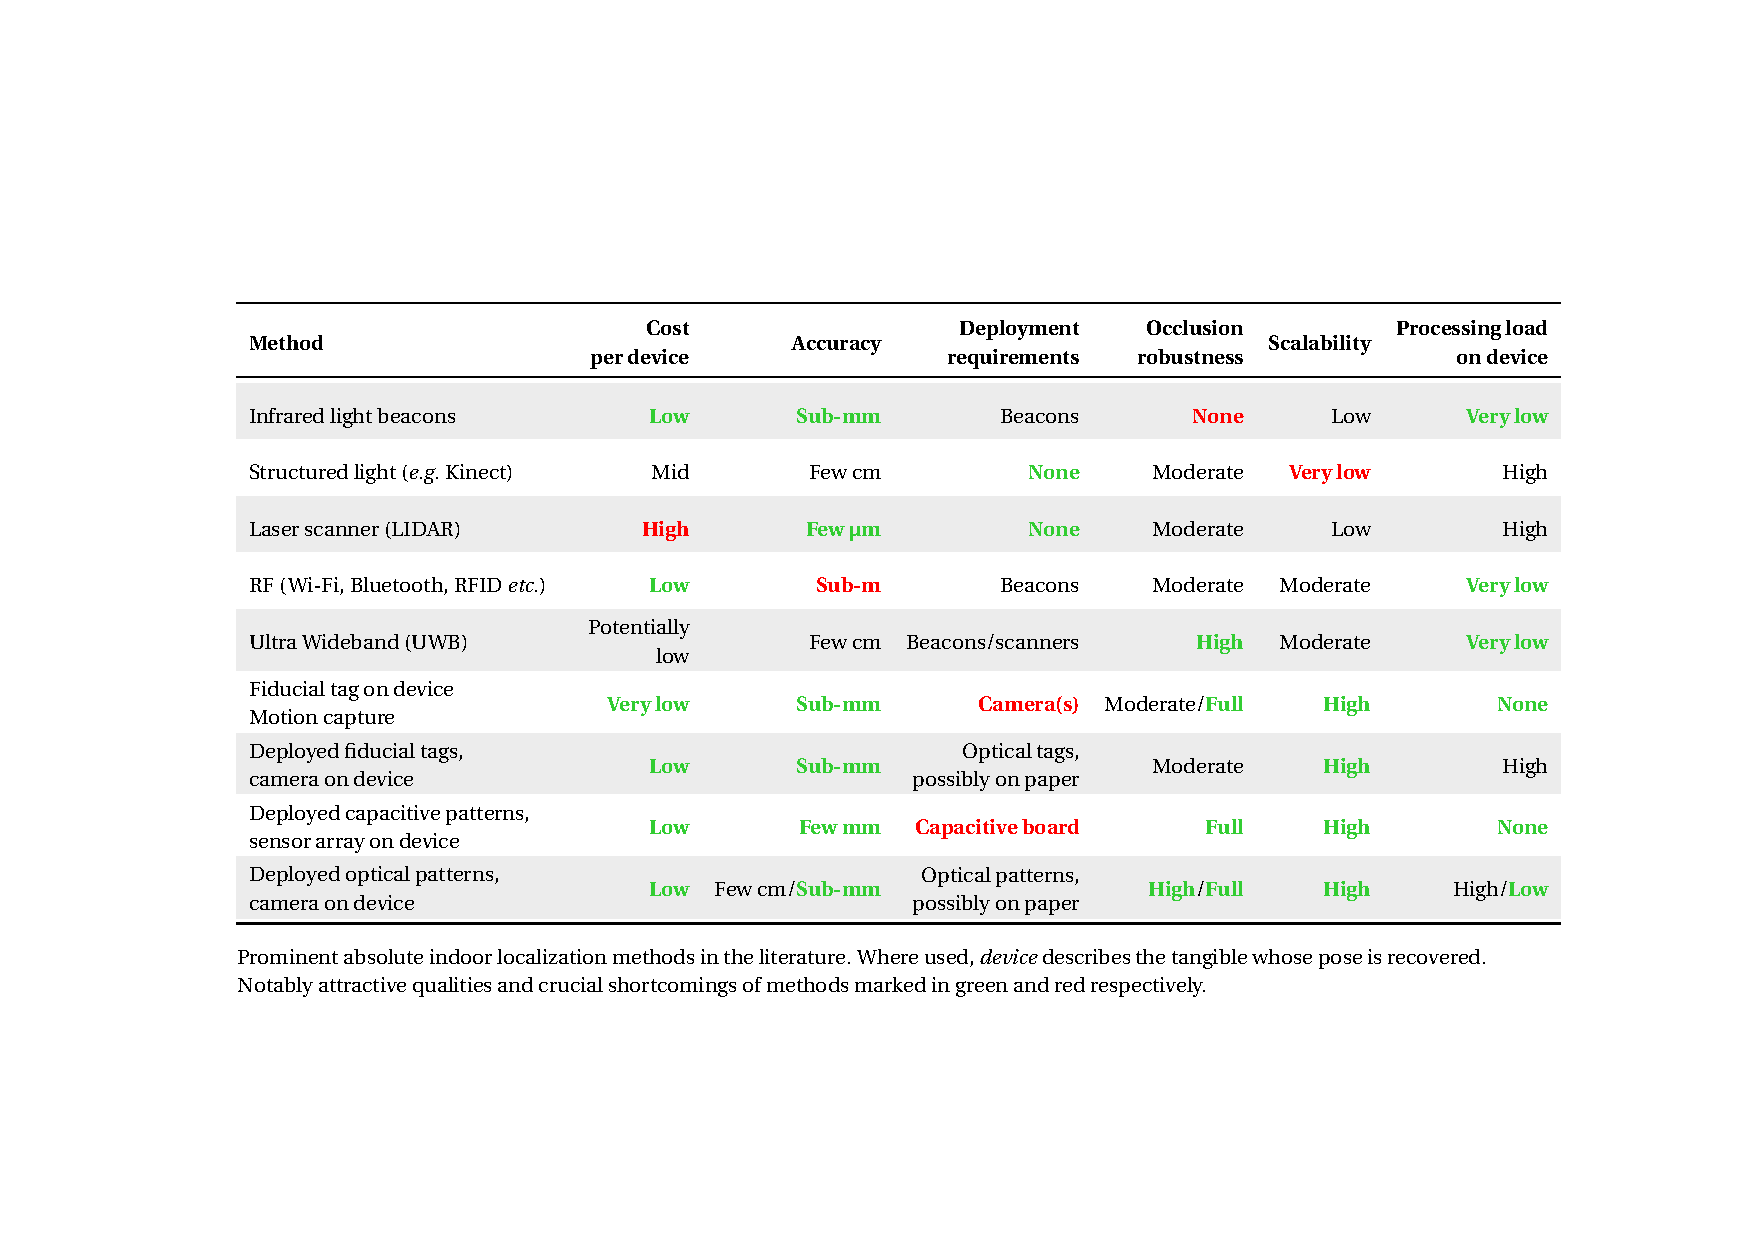
\includepdf{Prominent-absolute-indoor-localization-methods-comparison.pdf} 

% Please add the following required packages to your document preamble:
% \usepackage[table,xcdraw]{xcolor}
% If you use beamer only pass "xcolor=table" option, i.e. \documentclass[xcolor=table]{beamer}
% \usepackage{lscape}
\begin{landscape}
    \begin{table}[]
    \centering
    \begin{tabular}{lllllll}
    \hline
    Method                                                                                         & Cost per device & Accuracy      & \begin{tabular}[c]{@{}l@{}}Deployment\\ requirements\end{tabular}             & \begin{tabular}[c]{@{}l@{}}Occlusion\\ robustness\end{tabular} & Scalabiity & \begin{tabular}[c]{@{}l@{}}Processing load\\ on device\end{tabular} \\ \hline
    \rowcolor[HTML]{EFEFEF} 
    Infrared light beacons                                                                         & Low             & Sub-mm        & Beacons                                                                       & None                                                           & Low        & Very low                                                            \\
    Structured light (e.g. Kinect)                                                                 & Mid             & Few cm        & None                                                                          & Moderate                                                       & Very low   & High                                                                \\
    \rowcolor[HTML]{EFEFEF} 
    Laser scanner (LIDAR)                                                                          & High            & Few µm        & None                                                                          & Moderate                                                       & Low        & High                                                                \\
    \begin{tabular}[c]{@{}l@{}}RF (Wi-Fi, \\ Bluetooth, RFID etc.)\end{tabular}                    & Low             & Sub-m         & Beacons                                                                       & Moderate                                                       & Moderate   & Very low                                                            \\
    \rowcolor[HTML]{EFEFEF} 
    \begin{tabular}[c]{@{}l@{}}Ultra Wideband \\ (UWB)\end{tabular}                                & Potentially low & Few cm        & Beacons/scanners                                                              & High                                                           & Moderate   & Very low                                                            \\
    \begin{tabular}[c]{@{}l@{}}Fiducial tag on device\\ Motion capture\end{tabular}                & Very low        & Sub-mm        & Camera(s)                                                                     & Moderate/Full                                                  & High       & None                                                                \\
    \rowcolor[HTML]{EFEFEF} 
    \begin{tabular}[c]{@{}l@{}}Deployed fiducial tags,\\ camera on device\end{tabular}             & Low             & Sub-mm        & \begin{tabular}[c]{@{}l@{}}Optical tags, \\ possibly on paper\end{tabular}    & Moderate                                                       & High       & High                                                                \\
    \begin{tabular}[c]{@{}l@{}}Deployed capacitive patterns,\\ sensor array on device\end{tabular} & Low             & Few mm        & Capacitive board                                                              & Full                                                           & High       & None                                                                \\
    \rowcolor[HTML]{EFEFEF} 
    \begin{tabular}[c]{@{}l@{}}Deployed optical patterns,\\ camera on device\end{tabular}          & Low             & Few cm/Sub-mm & \begin{tabular}[c]{@{}l@{}}Optical patterns,\\ possibly on paper\end{tabular} & High/Full                                                      & High       & High/Low                                                            \\ \hline
    \end{tabular}
    \caption{Prominent absolute indoor localization methods in the literature. Where used, device describes the tangible whose pose is recovered. }
    \label{tab:localization}
    \end{table}
\end{landscape}

各类定位方法优缺点\cite{ozgur2018cellulo}如表~\ref{tab:localization}所示。

\subsection{底盘}
考虑到交互过程中需要推动小车,通过用户调查我们知道:大多数用户(特别是儿童)习惯于按压着移动小车,这就使得我们不能采用Zooids\cite{le2016zooids}(如图~\ref{fig:Zooids})或e-puck\cite{mondada2009puck}(如图~\ref{fig:e-puck})使用的差速转向,只能采用类似Cellulo\cite{ozgur2017cellulo}(如图~\ref{fig:Cellulo})的磁驱技术或WolfBot\cite{betthauser2014wolfbot}(如图~\ref{fig:WolfBot})使用的全向轮。

\begin{figure}[htbp]
    \centering
    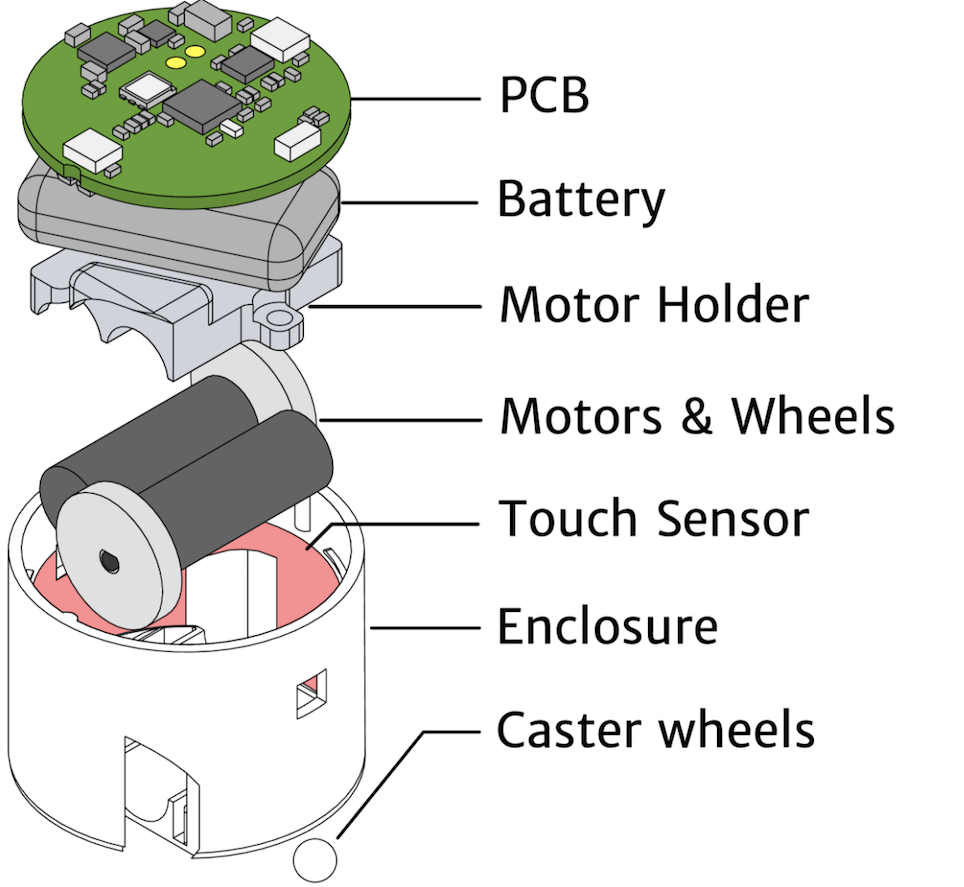
\includegraphics[height=10cm]{Zooids.png}
    \caption{Zooids}
    \label{fig:Zooids}
\end{figure}

\begin{figure}[htbp]
    \centering
    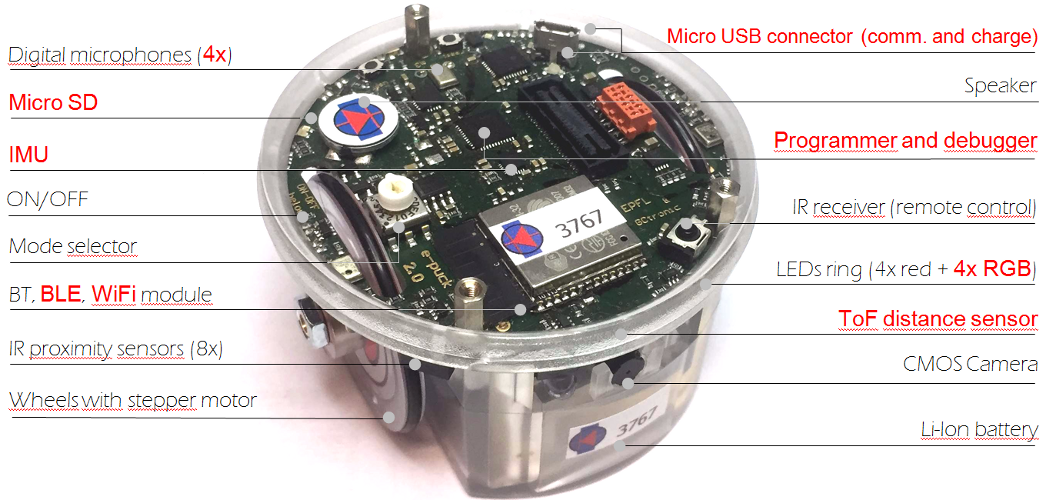
\includegraphics[height=6cm]{e-puck2-features_small.png}
    \caption{Zooids}
    \label{fig:e-puck}
\end{figure}

\begin{figure}[htbp]
    \centering
    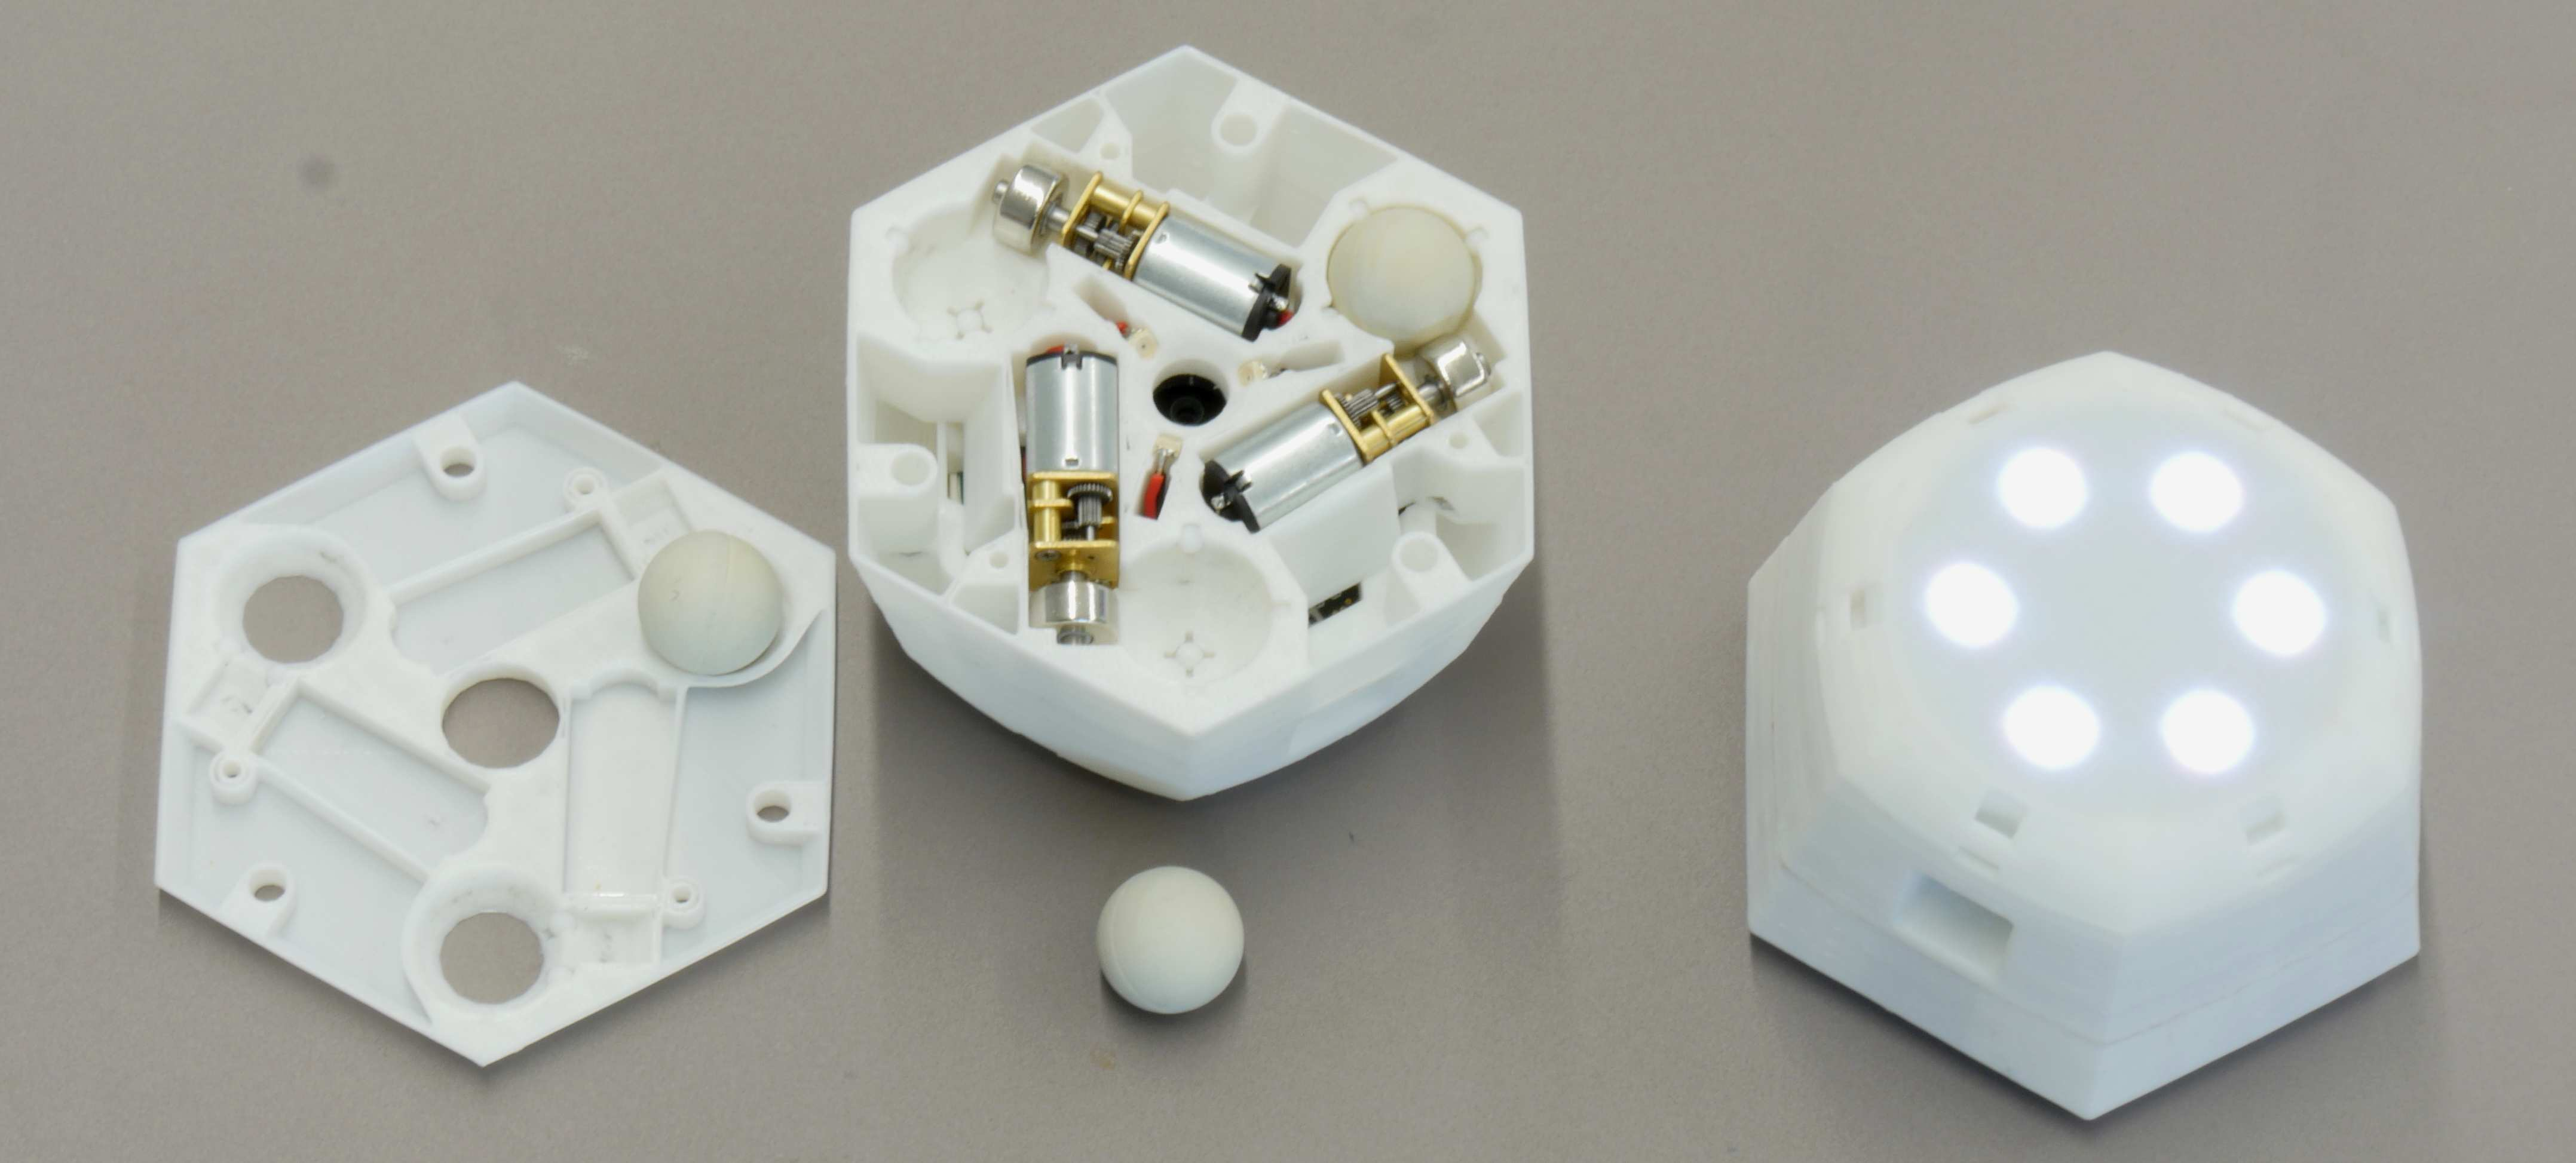
\includegraphics[height=6cm]{cellulo.jpg}
    \caption{Cellulo}
    \label{fig:Cellulo}
\end{figure}
  
\begin{figure}[htbp]
    \centering
    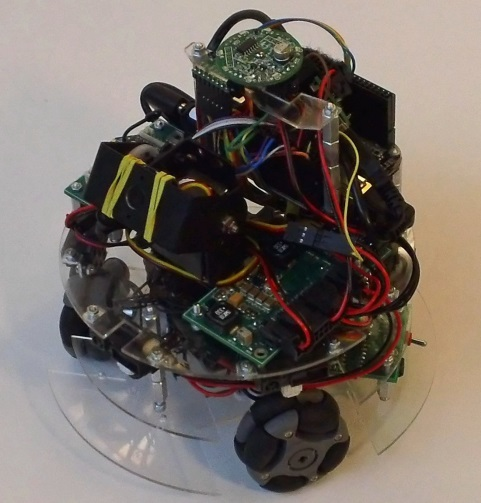
\includegraphics[height=10cm]{WolfBot.jpg}
    \caption{WolfBot}
    \label{fig:WolfBot}
\end{figure}

经过尝试,我们发现磁驱电机的速度和磁环的磁性强弱、电池的电量剩余、磁环和轴之间的胶合强度等不可控因素关系很大,无法建立起小车各轮速度和电机PWM占空比之间的时不变映射关系,导致很难控制小车的走向和速度,最终放弃了这一想法。

WolfBot采用的全向轮和电机直接连接,使得底盘占地面积很大。最终我们则采用1.5英寸麦克纳姆轮和GW12-N20减速电机(减速齿轮中的蜗杆改变90度传动方向)实现系统最小化。

\subsection{主控板}

\subsection{扩展接口}

\subsection{实物可视化界面}

\subsection{UI}